\documentclass[aspectratio=169]{beamer}\usepackage[utf8]{inputenc}
\usepackage[english]{babel}
\usepackage{color}
\usepackage{amsmath,mathtools}
\usepackage{mathptmx}
\usepackage[11pt]{moresize}
\setbeamertemplate{navigation symbols}{}
\setbeamersize{text margin left=5mm,text margin right=5mm}
\usepackage{wrapfig}
\usepackage{bbm}
\usepackage{xcolor}
\usepackage{tabularx}
\usepackage{bm}
\usepackage{lmodern}


\newcommand{\R}{\mathbb{R}}
\newcommand{\E}{\mathbb{E}}
\newcommand{\N}{\mathbb{N}}
\newcommand{\Z}{\mathbb{Z}}
\newcommand{\V}{\mathbb{V}}
\newcommand{\Q}{\mathbb{Q}}
\newcommand{\K}{\mathbb{K}}
\newcommand{\C}{\mathbb{C}}
\newcommand{\T}{\mathbb{T}}
\newcommand{\I}{\mathbb{I}}

\setbeamertemplate{caption}[numbered]

\title{On the Uncertainty of Wind Power Generation\\ continuous report}
\subtitle{ Waleed Alhaddad}

\begin{document}
\setbeamercolor{background canvas}{bg=blue!1}


\begin{frame}
\titlepage
\end{frame}

% \begin{frame}[label=guide]\frametitle{ Reader's Guide }
% List of changes in this iteration:
% \begin{itemize}
% \item Removed the term $p(1-p)$ from the model.
%     \begin{itemize}
%         \item derived the new ODE for the moments.
%         \end{itemize}
% \item Non-academic poster prepared.
% \end{itemize}
% Next steps:
% \begin{itemize}
% \item The french data set
%     \begin{itemize}
%         \item Organize and clean.
%     \end{itemize}
% \item Check the performance of the optimization.
%
% \end{itemize}
% \small{
% Note :
% \begin{itemize}
% \item Green slides: possible future extensions
% \item Red slides: notes to be removed
% \end{itemize}
% }
% \end{frame}

\begin{frame}\frametitle{ Base Model }
Moments approach with a Beta proxy. The SDE is given by
		\begin{equation}
		\begin{split}
		dV_t &=  - \theta_t V_t \  dt + \sqrt{2 \theta_t \alpha (V_t +p_t ) (1-V_t-p_t)} \  dW_t  \\ %\quad t > 0
		V_0 & = v_0
	\end{split}\label{VtSDE}
	\end{equation}
		and the moments by,
		\begin{equation*}
		\frac{d m_1 (t)}{dt} = - m_1(t)\theta_t \implies m_1(t_2)= V_{t_1} e^{-\int_{t_1}^{t_2} \theta_t \ dt }
		\end{equation*}
		\begin{equation*}
		\begin{split}
		\frac{d m_2 (t)}{dt} &=  - m_2(t)\theta(1+\alpha) + \alpha\theta m_1(t)( (1-p_t -p_t^2)) +2 \\
		& \implies m_2(t_2) = v_{t_1}^2 e^{-(1+\alpha)\int_{t_1}^{t_2} \theta_t \ dt} \\
		& \quad \quad + \alpha \int_{t_1}^{t_2} \left(\theta_s m_1(s)( 1-p_s - p_s^2 )+2\right)   e^{-(1+\alpha)\int_{t_1}^{t_2-s} \theta_u \ du}  \ ds
		\end{split}
		\end{equation*}
\end{frame}


\begin{frame}\frametitle{ solving for the moments numerically }
We discretize and integrate numerically step-by-step using  Euler,
\begin{align*}
  m_{1,i+1}&= v_i \ e^{ - \theta_i \Delta t} \\
  m_{2,i+1} &= \frac{v_i^2  + 2 \Delta t v_i  \alpha \theta_i p_i (1-p_i)(1-2p_i)  \alpha \theta_i p_i^2 (1-p_i)^2}{1+ 2 \Delta t (\theta_i + \alpha \theta_i p_i (1-p_i))}
\end{align*}
\end{frame}

\begin{frame}\frametitle{ Proposed Mini-Batch Stochastic Gradient Descent }
We have the following beta log-likelihood,
\begin{equation*}
\ell ( \theta_0 , \alpha | \{V_{i,j}\}) = \sum\limits_{j=1}^M \sum\limits_{i=1}^N \ (s_1 -1 ) \log \left( \frac{V_{j,i+1}+1}{2} \right) +  (s_2 -1 ) \log \left( 1 - \frac{V_{j,i+1}+1}{2} \right) - \log\left( 2 B(s_1, s_2) \right)
\end{equation*}
where $B(\cdot, \cdot)$ is the Beta function and
\begin{equation}
s_1 = - \frac{ (m_1+1)(m_1^2 + m_2 - m_1^2  -1 )}{2(m_2 - m_1^2)}
\end{equation}
\begin{equation}
s_2 = \frac{(m_1-1)(m_1^2 + m_2 - m_1^2  -1 )}{2(m_2 - m_1^2)}
\end{equation}
\end{frame}


\begin{frame}\frametitle{ 10 min data interval results }
We optimize the likelihood using Nelder-Mead Method which is a derivative-free method for non-linear objectives.
\begin{figure} %[t]
\begin{center}
%\fbox{\rule{0pt}{2in} \rule{0.9\linewidth}{0pt}}
\includegraphics[width=0.3\linewidth]{plots_SGD/ISO_100_inter=427.pdf}
\includegraphics[width=0.3\linewidth]{plots_SGD/ISO_500_inter=427.pdf}
\includegraphics[width=0.3\linewidth]{plots_SGD/ISO_833_inter=427.pdf}
\end{center}
   \caption{Likelihood evaluation with different number of sample paths. Optimal point $(\theta_0^*, \alpha^*) = (22.33,  0.049)$ shown in blue obtained using Nelder-Mead optimization method.}
\label{samples}
\end{figure}
\end{frame}


\begin{frame}\frametitle{ 10 min data interval results  }
\begin{figure} %[t]
\begin{center}
%\fbox{\rule{0pt}{2in} \rule{0.9\linewidth}{0pt}}
\includegraphics[width=0.6\linewidth]{plots_SGD/ISO_173_inter=427.pdf}
\end{center}
   \caption{Likelihood evaluation with 173 paths. Optimal point $(\theta_0^*, \alpha^*) = (22.33,  0.049)$ shown in blue obtained using Nelder-Mead optimization method.}
\label{100samples}
\end{figure}
\end{frame}


\begin{frame}\frametitle{ 10 min data interval results  }
\begin{figure} %[t]
\begin{center}
%\fbox{\rule{0pt}{2in} \rule{0.9\linewidth}{0pt}}
\includegraphics[width=0.8\linewidth]{plots_SGD/0.pdf}
\end{center}
   \caption{ Example 24hr simulation paths with the optimal parameters $(\theta_0^*, \alpha^*) = (22.33,  0.049)$}
\label{100samples}
\end{figure}
\end{frame}
\begin{frame}\frametitle{ 10 min data interval results  }
\begin{figure} %[t]
\begin{center}
%\fbox{\rule{0pt}{2in} \rule{0.9\linewidth}{0pt}}
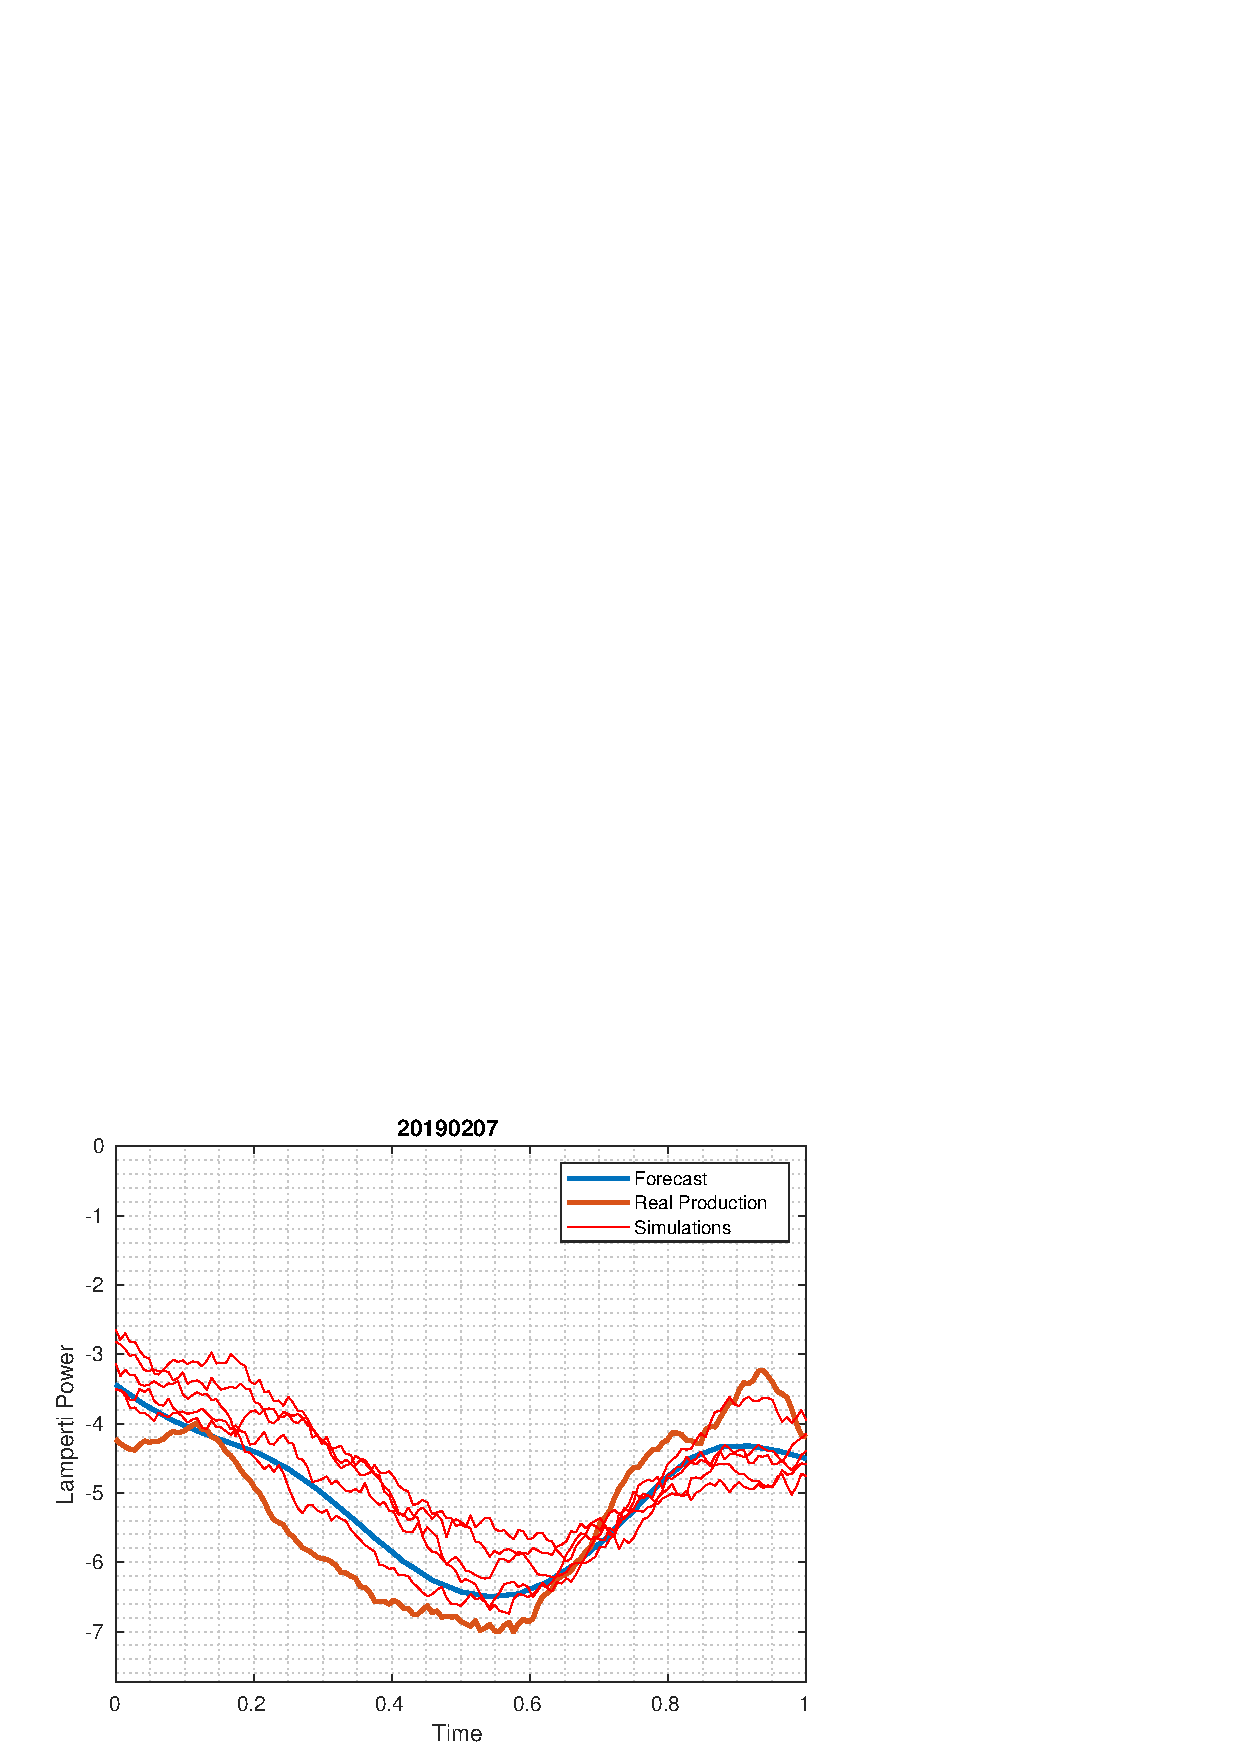
\includegraphics[width=0.8\linewidth]{plots_SGD/18.pdf}
\end{center}
   \caption{ Example 24hr simulation paths with the optimal parameters $(\theta_0^*, \alpha^*) = (22.33,  0.049)$}
\label{100samples}
\end{figure}
\end{frame}
\begin{frame}\frametitle{ 10 min data interval results  }
\begin{figure} %[t]
\begin{center}
%\fbox{\rule{0pt}{2in} \rule{0.9\linewidth}{0pt}}
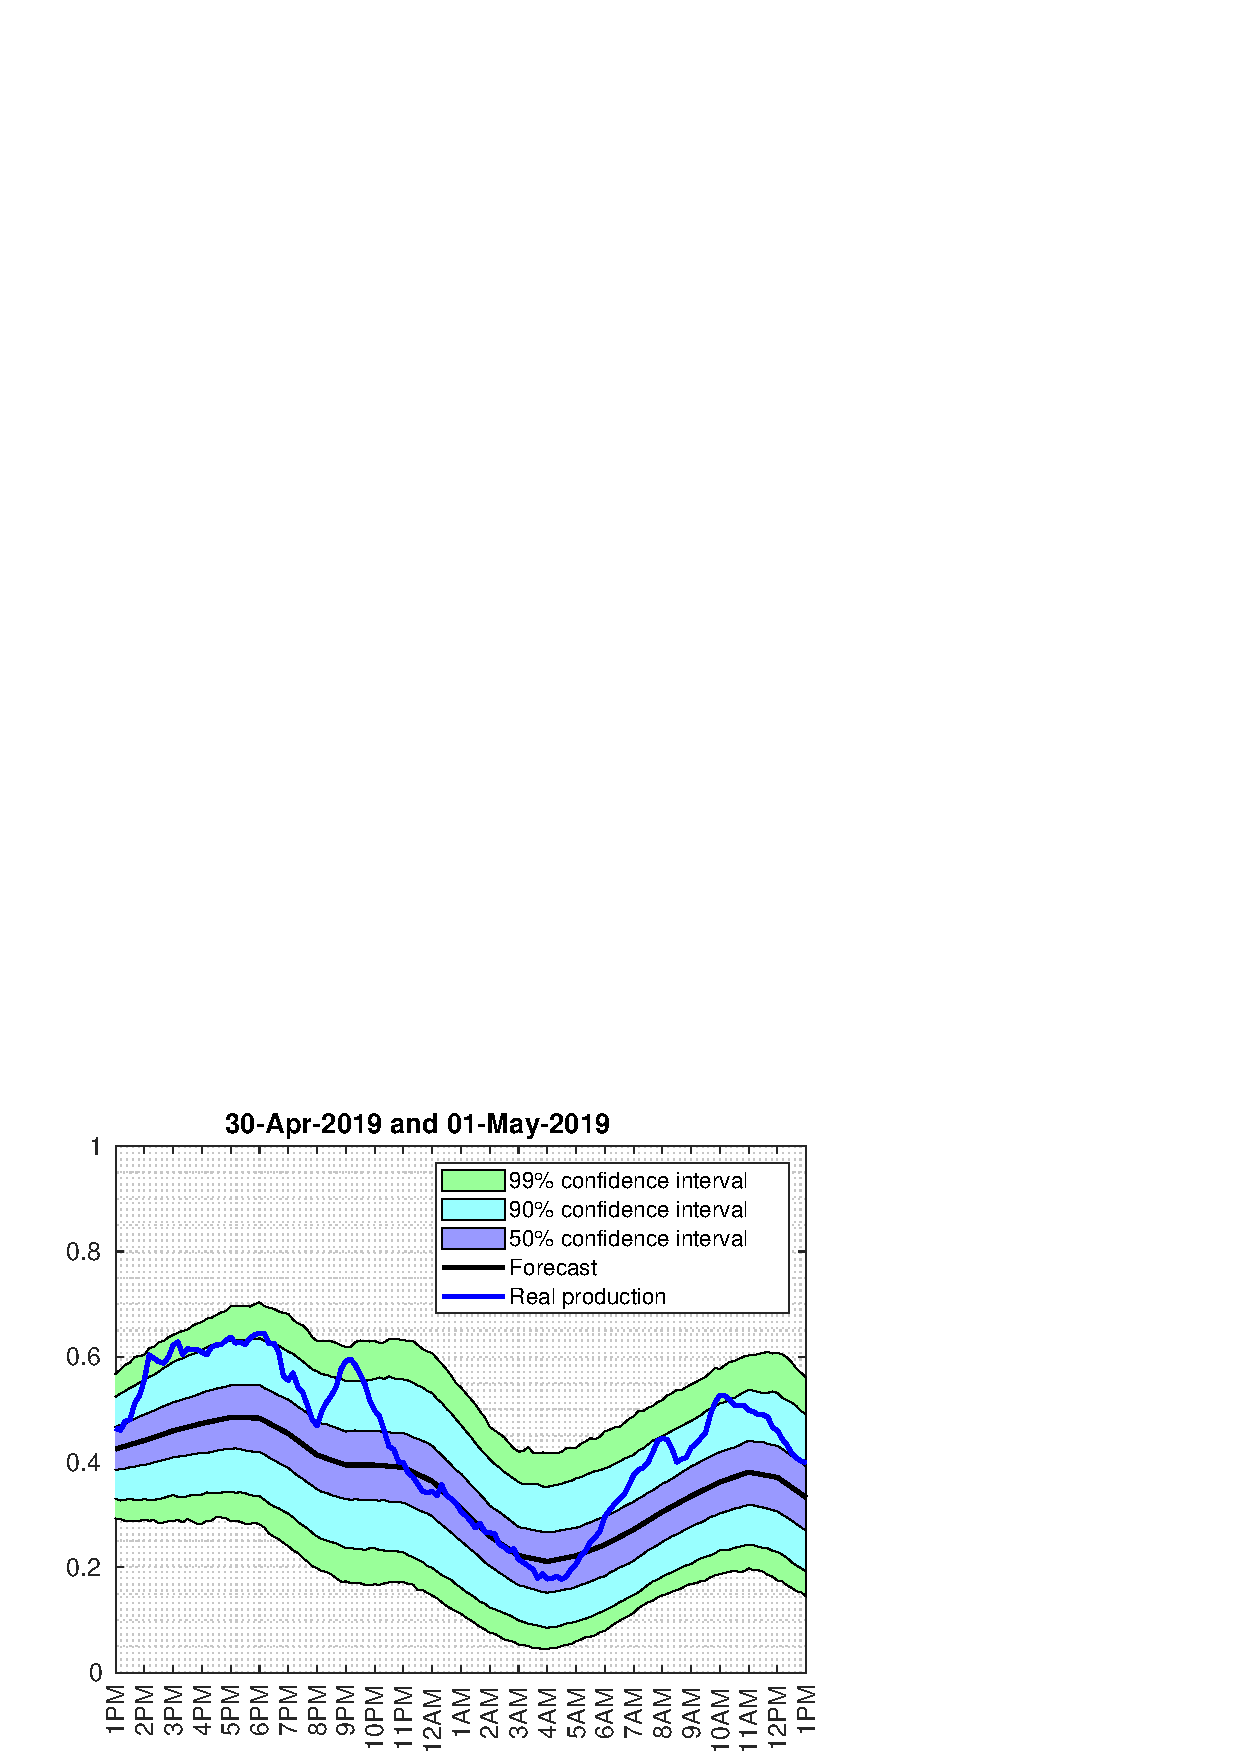
\includegraphics[width=0.8\linewidth]{plots_SGD/4.pdf}
\end{center}
   \caption{ Example 12hr simulation paths with the optimal parameters $(\theta_0^*, \alpha^*) = (22.33,  0.049)$}
\label{100samples}
\end{figure}
\end{frame}
\begin{frame}\frametitle{ 10 min data interval results  }
\begin{figure} %[t]
\begin{center}
%\fbox{\rule{0pt}{2in} \rule{0.9\linewidth}{0pt}}
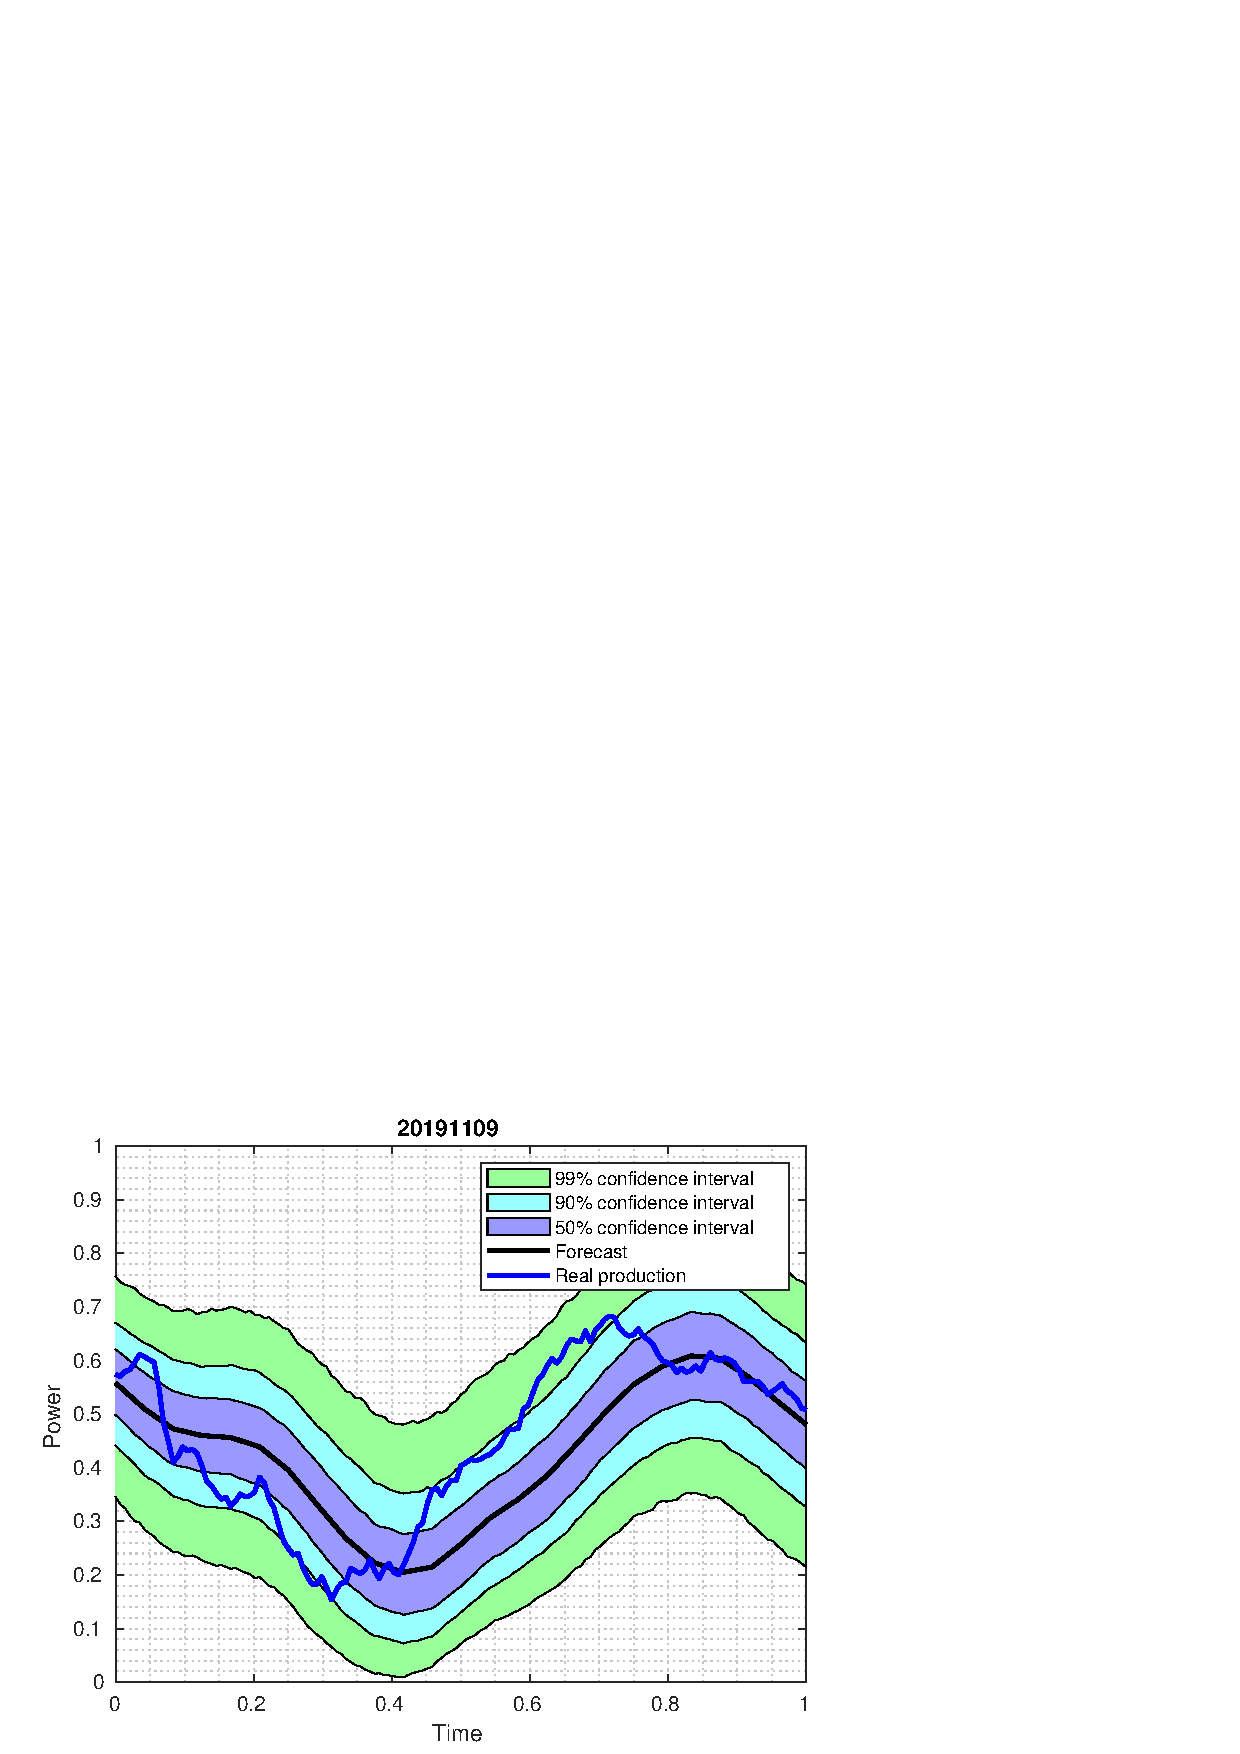
\includegraphics[width=0.8\linewidth]{plots_SGD/105.pdf}
\end{center}
   \caption{ Example 12hr simulation paths with the optimal parameters $(\theta_0^*, \alpha^*) = (22.33,  0.049)$}
\label{100samples}
\end{figure}
\end{frame}

\begin{frame}\frametitle{ Proposed Mini-Batch Stochastic Gradient Descent }
Let $B$ be the mini-batch size and $\eta$ the learning rate.\\

We iterate from an initial guess $\Theta_0 = (\theta_0 , \alpha)^T$ in the following way,
\begin{equation}
  \Theta = \Theta  - \eta \nabla \ell  \left( \Theta ; V_{1:B, 1:N} \right)
\end{equation}

until an accuracy threshold is reached. Note that $V_{1:B, 1:N}$ is a mini-batch of size $B$ of complete sample paths. The components of the gradient $\nabla \ell = (\frac{\partial \ell }{\partial \theta_0},\frac{\partial \ell}{\alpha} )^T$ are given by,

\begin{equation*}
\frac{\partial \ell }{\partial \theta_0} = \frac{\partial \ell }{\partial s_1}\frac{\partial s_1 }{\partial m_1}\frac{\partial m_1 }{\partial \theta_t}\frac{\partial \theta_t }{\partial \theta_0} + \frac{\partial \ell }{\partial s_1}\frac{\partial s_1 }{\partial m_2}\frac{\partial m_2 }{\partial \theta_t}\frac{\partial \theta_t }{\partial \theta_0} + \frac{\partial \ell }{\partial s_2}\frac{\partial s_2 }{\partial m_1}\frac{\partial m_1 }{\partial \theta_t}\frac{\partial \theta_t }{\partial \theta_0} + \frac{\partial \ell }{\partial s_2}\frac{\partial s_2 }{\partial m_2}\frac{\partial m_2 }{\partial \theta_t}\frac{\partial \theta_t }{\partial \theta_0}
\end{equation*}

\begin{equation*}
\frac{\partial \ell }{\partial \alpha} =  \frac{\partial \ell }{\partial s_1}\frac{\partial s_1 }{\partial m_2}\frac{\partial m_2 }{\partial \alpha} + \frac{\partial \ell }{\partial s_2}\frac{\partial s_2 }{\partial m_2}\frac{\partial m_2 }{\partial \alpha}
\end{equation*}

\end{frame}


\begin{frame}\frametitle{Proposed Mini-Batch Stochastic Gradient Descent}
We run into an issue here because the term $ \frac{\partial \theta_t }{\partial \theta_0} $ is undefined as $\theta_t$ is non-differentiable and given by,
\begin{equation*}
  \theta_t = \max \left( \theta_0 , \frac{ |\dot{p}| }{ \min (p, 1-p)} \right)
\end{equation*}

We can either regularize or continue to use the Nelder-Mead optimization method which is derivative-free. Is it possible to use mini-batches with Nelder-Mead?

\end{frame}


% \begin{frame}\frametitle{ Proposed Mini-Batch Stochastic Gradient Descent }
%  We differentiate with respect to the parameters:
% \begin{equation}
%   J_{s_1}^M\left( s_1, s_2 ; V_{1:M, 1:N} \right)=\frac{\partial \ell}{ \partial \alpha } = \sum\limits_{j=1}^M \sum\limits_{i=1}^N \  \log \left( \frac{V_{j,i+1}+1}{2} \right) - \psi(s_1) + \psi(s_1 + s_2)
% \end{equation}
% \begin{equation}
%   J_{s_2}^M \left( s_1, s_2 ; V_{1:M, 1:N} \right) =\frac{\partial \ell}{ \partial \beta } = \sum\limits_{j=1}^M \sum\limits_{i=1}^N \  \log \left(1-  \frac{V_{j,i+1}+1}{2} \right) - \psi(s_2) + \psi(s_1 + s_2)
% \end{equation}
% % \begin{equation}
% %   \nabla_{\alpha,\beta} J \left( \Theta ; V_{1:M, 1:N} \right) = \frac{\partial \ell}{ \partial \alpha \partial \beta } = \frac{\partial \ell}{ \partial \beta \partial \alpha  }= M N \ \psi^{(1)} (\alpha + \beta)
% % \end{equation}
% %$\psi^{(1)}(\cdot)$ is the trigamma function.
% where $\psi(\cdot)$ is the digamma function.
% \end{frame}



%\againframe{guide}



\end{document}
